\chapter{Introduction}
\label{Introduction}
The following master's thesis takes its starting point in the use of user involvement product development in a company. Whether this means conducting extensive user studies or simply applying feedback from the users in the design process, it has multiple benefits...

The significance of involving users in the design process of any product is considered beneficial from the viewpoint of people working in the field of user experience design. It is also a growing trend amongst developers not usually applying user involvement (sovs? - Øvad).

%Why apply user involvement in product development? (Strengths)
%	- satisfied customers
%	- Decreased training and support costs
%		(In the perfect scenario, the system provides the necessary informations on its own. 	 e.g. Don Norman, system image, conceptual modelling etc.)
%	- Reduced development time and costs
%	- Decreased user errors

%The definition / Examples of user involvment
%	- The definition of UX and usability
%	- They are often perceived as the same - Tina considers UX a broader, superior field which includes usability.

%Consequently the focus on UX-design has increased within industry in recent years (Current weaknesses)
%	- However there is a "gap between academic and industry" - Hvad skyldes det, og hvordan gøres det "gap" mindre?
%	- This difference lies in how UX methods are developed in an academic scenario and subsequently employed in the industry.
%	- "The litterature evaluating usability methods is fundamentally flawed by its lack of relevance to applied usability work"
%	- User experience is still a new and fresh concept to many companies.

%Our intention, on the basis of this, is to investigate its relevance for a specific case - a specific company: TC Electronic
%	- Brief presentation of who TC Electronic are - and how we got to work with them
%	- More specifically the focus is on the TonePrint community - It is something they currently need, and as such it made sense to focus on it.
%	- The TonePrint concept

%Research question
%	- How will this be investigated?
%	- The level of involvement from TC Electronic









%The following master's thesis takes its starting point in the TonePrint concept from TC Electronic (from here on referred to as \textit{TC}). Its reveal in 2011 opened a new playground for musicians and tone tweakers, making effect editing possible from the users smartphone. Until this point, TC was already a worldwide known manufacturer of effect pedals for guitarists, originally formed in the early 1970's by Kim and John Rishøj in Aarhus, Denmark. With this as the baseline for the thesis, the focus will be on the future for this concept, starting with a general description of effect units and the capabilities of TonePrints.
%
%\section{The TonePrint Concept}
%\label{TonePrints}
%Effect pedals in general are well known units for guitarists and bassists alike, spanding multiple music genres. The pedal works by taking the input signal from the guitar and changing it to the tweaking by the users. Depending on the effect type, and when playing, the user activates these changes by a single button on the pedal. An example of a simple guitar effect pedal is displayed on \autoref{fig:EffectPedalExample}, where the adjustable parameters on it consists of \textit{Dwell, Mix,} and \textit{Tone}. Each of these are accessed and tweaked with individual knobs on the unit, which gives the user a limited range of ways to change the sound.
%
%With this limitation as a motivation, TC created the TonePrint concept, enabling users to tweak the sound of effects beyond the parameters on the pedals. Using the TonePrint application, the users have a vast selection of custom presets with further parameters available for tweaking. These presets are what the term \textit{TonePrint} covers and they are either created in collaboration with professional musicians or by the common user. In order to distinguish these from each other, they are referred to as \textit{Artist TonePrints} and \textit{User TonePrints} respectively. After selecting one for the effect pedal in question, the user can make any desired tweaking or transfer it directly to the pedal with the option of altering it even more on the physical knobs \parencite{PDF:TonePrintAnalyse}. TC has collaborated with multiple guitarists and bassists, creating TonePrints for effect pedals used by the artists themselves. After the creators are satisfied with their TonePrints, they are uploaded to the TonePrint library in the application where any users of the same effect pedal can download the TonePrint and as such match the sound of their favourite artist. For User TonePrints the overall concept is the same. They differ in the fact that the creator isn't a famous guitarist, but the TonePrint is still made using the application and can be transferred directly to its effect pedal. However, when it comes to sharing these User TonePrint with friends and other aspiring guitarist, a platform for this purpose doesn't exist yet.
%%
%\begin{figure}[H]
%	\centering
%	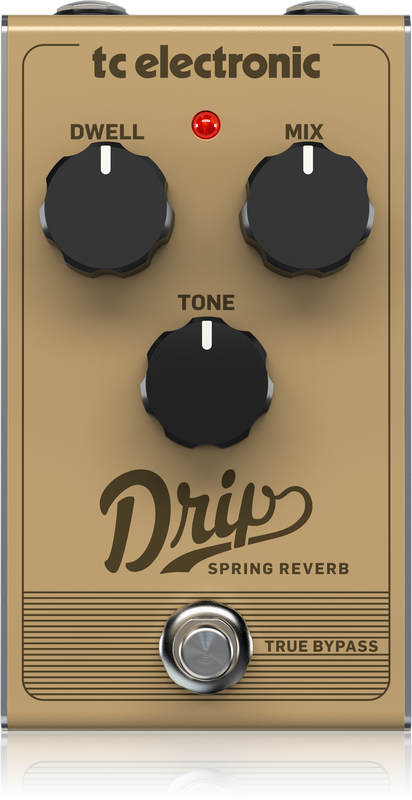
\includegraphics[width=.20\textwidth]{Graphics/EffectPedalExample}
%	 \caption{This figure shows a Drip spring reverb effect pedal by TC Electronics \url{https://www.tcelectronic.com/Categories/Tcelectronic/Guitar/Stompboxes/DRIP-SPRING-REVERB/p/P0CQ2\#googtrans(en|en)}.}
%    \label{fig:EffectPedalExample}
%\end{figure}
%%
%\subsection{The TonePrint Software}
%\label{TonePrintSoftware}
%As previously stated, the exploring of TonePrints start with the TonePrint application available for smartphones and tablets. However, the software is also available for PC and MAC, and the reason for this distinction lies in the difference of how a TonePrint is transferred to its respective pedal. For PC and MAC the user is required to use a cable from the computer to the pedal, but through the tablet and smartphone application, the user also have the option of simply beaming it directly to the pedal. whatever the platform, however, when opening the software the user is introduced to a list selection of different effect pedals, each holding a vast number of TonePrints created by famous guitarists. After selecting an effect pedal from this list, the user is then presented a new list selection of the many guitarist who have created TonePrints for this pedal. When selecting one of the guitarists, and depending on whether the guitarist have created more TonePrints for the same pedal, the user is then presented a bigger view of this specific TonePrint with a description of it and its creator. An example of this is displayed on \autoref{fig:TonePrintAppExample}. Depending on the users' motivation when opening the application first time, they can also choose to browse by artist instead of pedal, if their starting point is to find out what it takes to sound like their favourite artist.
%
%\begin{figure}[H]
%	\centering
%	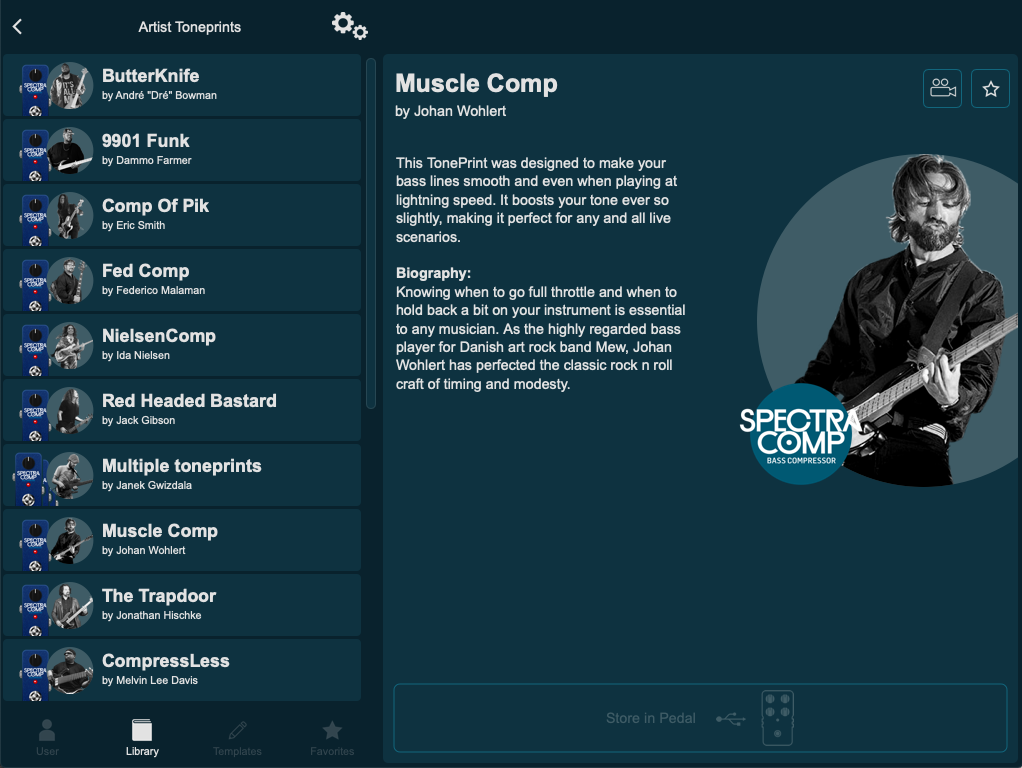
\includegraphics[width=\textwidth]{TonePrintAppExample}
%	\caption{The view in the TonePrint application after selecting an effect pedal and a TonePrint. This example displays a TonePrint created by Johan Wohlert of the danish rock band \textit{Mew}.}
%	\label{fig:TonePrintAppExample}
%\end{figure}
%\noindent

%\begin{itemize}
%	\item Man kan overføre med kabel eller beaming\fxnote{Der skal laves henvisning til appen i sig selv}
%	\item If a user should attempt to transfer a TonePrint of an effect pedal to a completely different unit, it simply wouldn't work.
%	\item Et billede af appen, men hvad skal det billede helt præcist vise? Hvor i appen skal man være?\fxnote{Indsæt billede af appen}
%	\item Brugeren kan også starte med at browse ud fra guitarist i stedet for deal type => Det er ikke til at sige, hvad brugerens motivation er.
%    \item Brug en termologi som ikke kun forståes af musikere og overvej at forklare hvad toneprint er når det nævnes så man ikke skal læse mange linjer før en forklaring kommer.
%    \item overvej at omformulere den øverste "hat" eventuelt fjern den.
%    \item lav en tdligere skillelinje mellem artist og user toneprint.
%\end{itemize}

%\section{What should be in the introduction}
%\label{WhatShouldBeInTheIntroduction}
%
%\begin{itemize}
%	\item A short description of TC Electronic (Just the basics)
%	
%	\begin{itemize}
%		\item TC laver effektpedaler og er kendt på verdensplan
%		\item  A very short description of the principal of TonePrint (A later chapter/section will go more in depth \autoref{TonePrints}
%		\item Something about TC wanting to enable the users to share their UserTonePrints
%	\end{itemize}
%	
%	\item TC wish to include their users in the development of the new sharing platform (Community).
%	
%	\begin{itemize}
%		\item Hvorfor er det generelt en god ide at inddrage brugere til at løse designproblemer?
%		\item Hvad er typiske problemer?
%	\end{itemize}
%	
%	\item Something in general about how communities works and why it's important to include the users in the development of one.	
%	
%	\begin{itemize}
%		\item TC's Koncern community
%		\item Generelt ønske fra brugerne, at de gerne vil have et TonePrint community. - Det kræver kun et besøg på diverse fora for at finde dette ønske
%	\end{itemize}
%
%\end{itemize}


%Processen skal gå fra at TC har ønske om at lave et TonePrint Community. Det vi så skal arbejde hen imod er at finde ud af, hvordan en virksomhed som TC kan foretage brugerinddragelse, og hvordan de specifikt skal gøre det i forhold til dette.